\documentclass{article}
\usepackage{hyperref}
\usepackage{listings}
\usepackage{color}
\usepackage{xcolor}
\usepackage{geometry}
\usepackage{graphicx}
\usepackage{amsmath}
\usepackage{caption}
\usepackage{subcaption}
\usepackage[capitalise]{cleveref}
\usepackage{wrapfig}
\usepackage{amssymb}

\geometry{margin=1in}
\pdfminorversion=6

\newcommand\TODO[1]{\textcolor{red}{TODO: #1}}

\newcommand\header[2]{
    \begin{center}
        {\large
        UCSD CSE 167 Assignment #1: \\
        \vspace{0.3cm}
        \Large
        #2}
    \end{center}
}

\definecolor{dkgreen}{rgb}{0,0.6,0}
\definecolor{gray}{rgb}{0.5,0.5,0.5}
\definecolor{mauve}{rgb}{0.58,0,0.82}
\lstset{frame=tb,
        aboveskip=3mm,
        belowskip=3mm,
        showstringspaces=false,
        columns=flexible,
        basicstyle={\small\ttfamily},
        numbers=none,
        numberstyle=\tiny\color{gray},
        keywordstyle=\color{blue},
        commentstyle=\color{dkgreen},
        stringstyle=\color{mauve},
        breaklines=true,
        breakatwhitespace=true,
        tabsize=2
}

% Taken from https://tex.stackexchange.com/questions/83085/how-to-improve-listings-display-of-json-files

\colorlet{punct}{red!60!black}
\definecolor{delim}{RGB}{20,105,176}
\colorlet{numb}{magenta!60!black}

\lstdefinelanguage{json}{
    basicstyle=\normalfont\ttfamily,
    numberstyle=\scriptsize,
    stepnumber=1,
    numbersep=8pt,
    showstringspaces=false,
    breaklines=true,
    frame=lines,
    tabsize=2,
    literate=
     *{0}{{{\color{numb}0}}}{1}
      {1}{{{\color{numb}1}}}{1}
      {2}{{{\color{numb}2}}}{1}
      {3}{{{\color{numb}3}}}{1}
      {4}{{{\color{numb}4}}}{1}
      {5}{{{\color{numb}5}}}{1}
      {6}{{{\color{numb}6}}}{1}
      {7}{{{\color{numb}7}}}{1}
      {8}{{{\color{numb}8}}}{1}
      {9}{{{\color{numb}9}}}{1}
      {:}{{{\color{punct}{:}}}}{1}
      {,}{{{\color{punct}{,}}}}{1}
      {\{}{{{\color{delim}{\{}}}}{1}
      {\}}{{{\color{delim}{\}}}}}{1}
      {[}{{{\color{delim}{[}}}}{1}
      {]}{{{\color{delim}{]}}}}{1},
}

\hypersetup{colorlinks=true}


\begin{document}

\header{1}{3D Software Rendering}

The previous homework focused on 2D graphics (which is already quite important!). In this homework, we're going 3D. We will define shapes in 3D, project them onto the screen space, and render them. The projection is going to simulate how a camera (or our eyes) works: it 

\begin{figure}[h]
    \centering
    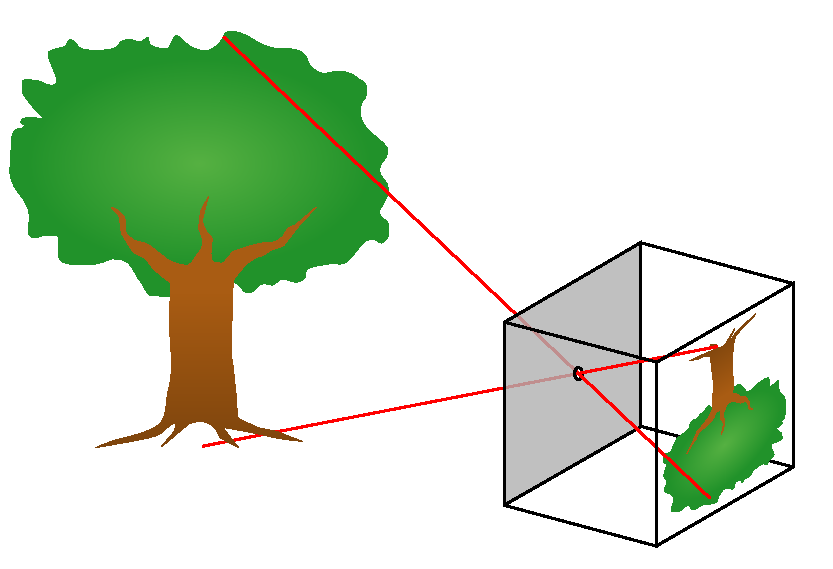
\includegraphics[width=0.5\linewidth]{imgs/pinhole.pdf}
    \caption{In this homework, we will implement 3D rendering by projecting 3D objects onto images. This is similar to a real-world camera. In particular, we will implement an ideal \href{https://en.wikipedia.org/wiki/Pinhole_camera}{pinhole camera}. Figure taken from \href{https://commons.wikimedia.org/wiki/File:Pinhole-camera.svg}{Wikipedia}.}
    \label{fig:pinhole}
\end{figure}

To facilitate the projection, we will focus on representing 3D surfaces, instead of the full volume. Instead of supporting multiple shapes (circles, squares, etc) like last time, we will focus on a single primitive: triangle. A main reason is that triangle has a very cool property: after perspective projection to 2D, it's still a triangle! (See \cref{fig:perspective}.) Many other shapes do not have this nice property -- a sphere projecting on to 2D can be an ellipse, a square projecting to the screen can become a general quadliteral.

\begin{figure}[h]
    \centering
    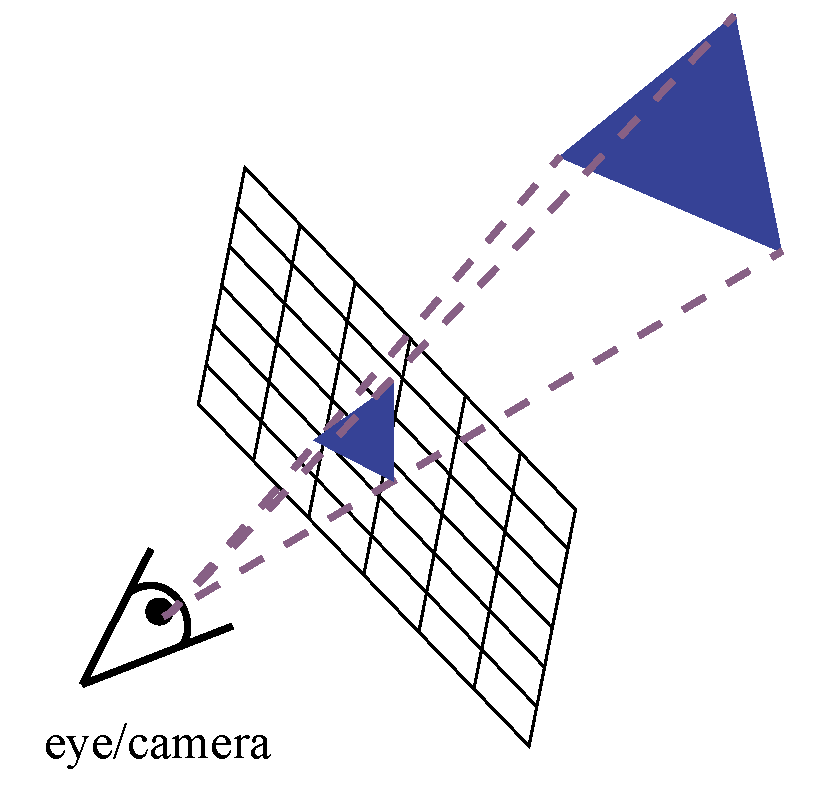
\includegraphics[width=0.5\linewidth]{imgs/perspective_projection.pdf}
    \caption{The perspective projection of a triangle.}
    \label{fig:perspective}
\end{figure}

\section{Rendering a single 3D triangle}
Let's start simple and render just a single 3D triangle. Our plan is to first project the triangle to a 2D image plane, then we can directly use the code from our previous homework to render the projected triangle.

\begin{figure}[h]
    \centering
    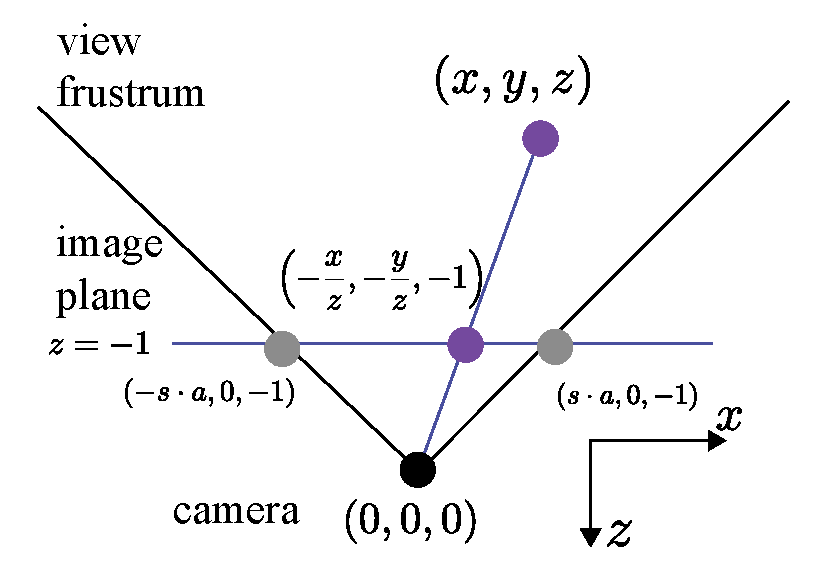
\includegraphics[width=0.5\linewidth]{imgs/perspective_transform.pdf}
    \caption{To perform perspective projection, we setup the coordinate system of the camera space so that the origin of the camera is at $(0, 0, 0)$, the camera is facing negative $z$-axis, $x$-axis is pointing right, and $y$-axis is pointing up. We put the image plane at $z=-z_0$. The perspective projection of a point $(x, y, z)$ is then simply finding the intersection between the line formed by the point and the camera origin with the image plane. Since our image plane has a finite extent, we further clips all point outside of $[-sa, -s, -z_0] \times [sa, s, -z_0]$ where $a$ is the aspect ratio ($\frac{\text{image width}}{\text{image height}}$) and $s$ is the scaling factor controlling the size of our image. The clipping defines a \emph{view frustrum}.}
    \label{fig:perspective_transform}
\end{figure}

How do we project the triangle then? It's significantly easier if we assume a particular coordinate system of our camera. We will lift this assumption in the later part of the homework (by, you guess it, applying 3D transformations). Let's assume in the \emph{camera space}, $x$-axis is pointing right, $y$-axis is pointing up, and $z$-axis is pointing away from the direction the camera is looking at. We also assume that the image plane is located at $z=-z_0$. \cref{fig:perspective_transform} shows that the perspective projection of a point $(x, y, z)$ boils down to computing the intersection between the line formed by the point and the camera origin with the image plane. The projected point $(x', y')$ is
\begin{equation}
\left(x', y'\right) = \left(-\frac{x}{z}, -\frac{y}{z}\right).
\label{eq:projection}
\end{equation}

Furthermore, we need to define the extent of the image plane (we can't have an image with infinite size!). Note that our image can be a rectangle (instead of a square). We define the extent of the image plane to be $[-sa, -s, -z_0] \times [sa, s, -z_0]$: $s$ is a scaling factor that controls the size of the image, and $a$ is the aspect ratio ($\frac{\text{image width}}{\text{image height}}$). As we will later show, $s$ is related to the \href{https://en.wikipedia.org/wiki/Field_of_view}{field of view} of a camera. Any point that lands outside of the extend of the image plane is discarded and not going to show up in our image. We call the set of points that are going to land on the image planes the \emph{view frustrum}. \cref{fig:perspective_transform} also visualizes the view frustrum.

Therefore, given a triangle with 3 vertices, we will project all three of them onto the image plane using \cref{eq:projection}. This generates a 2D triangle which we can then render using our previous homework's code.

\begin{figure}[h]
    \centering
    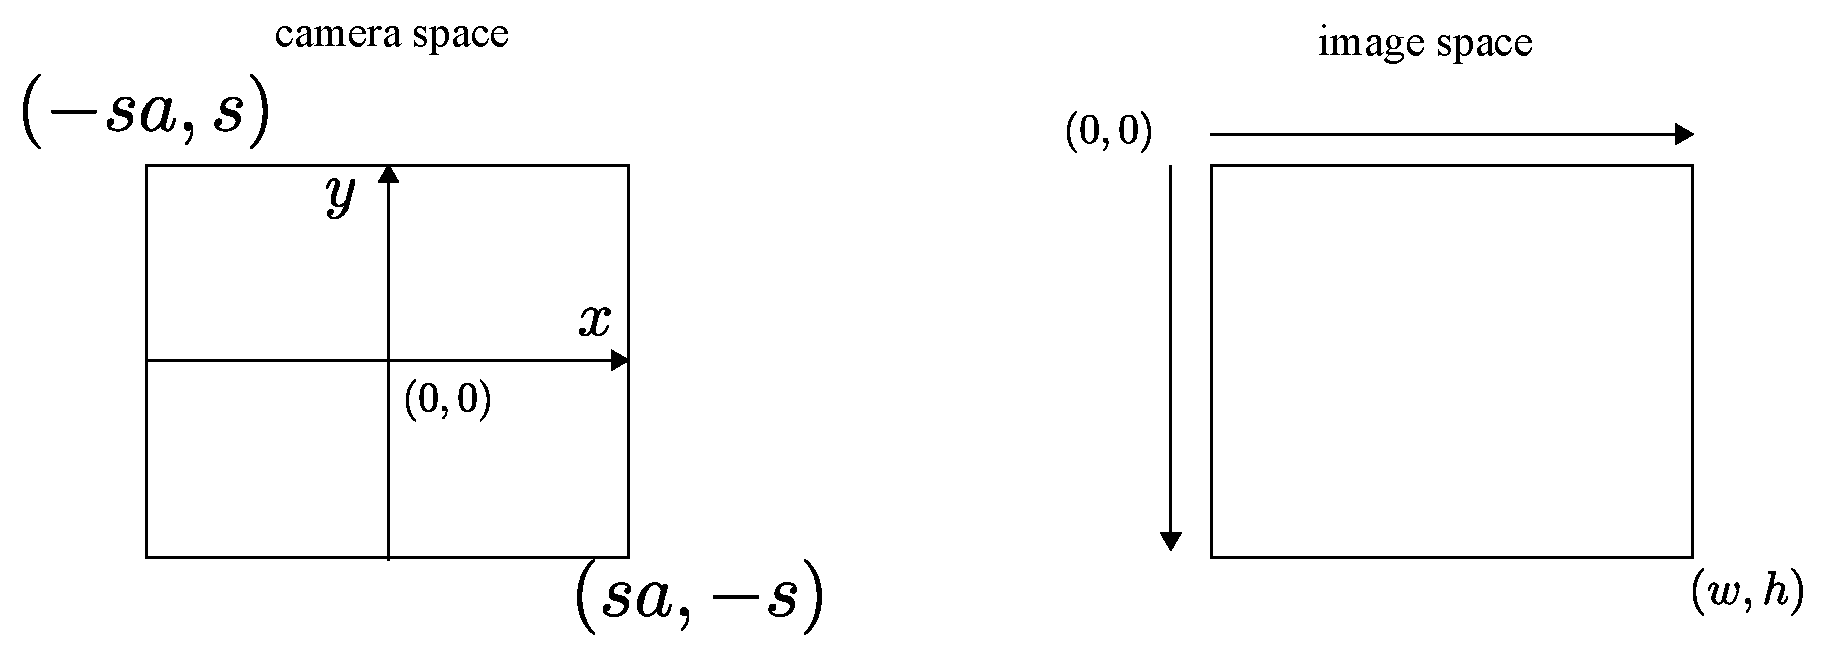
\includegraphics[width=0.9\linewidth]{imgs/camera_vs_image.pdf}
    \caption{The different coordinate systems between our camera space and image space.}
    \label{fig:camera_vs_image}
\end{figure}

There are a few other complications though. Firstly, the point $(x', y')$ is in the (projected) camera space after the projection. We will need to transform it into the screen space. Recall that our screen space has $x$-axis pointing right with $y$-axis pointing down, and the extent is $[0, 0] \times [\text{width}, \text{height}]$. See \cref{fig:camera_vs_image}. So we need to further convert the point $(x', y')$ from the projected camera space to image space. Looking at \cref{fig:camera_vs_image}, we can see that the we need to translate the origin, scale the axes, and flip the $y$ axis. We will give you the formula for the $x$-axis, and you should figure out the $y$-axis formula yourself:
\begin{equation}
x'' = w\frac{x'+sa}{2sa},
\end{equation}
where $w$ is the width of the image.

The second complication is that a triangle vertex can be behind the camera i.e., $z < 0$. In fact, even if $z$ is very close to zero, it can be still problematic: recall that in \cref{eq:projection}, we need to divide by $z$ for the projection. When $z$ is very close to zero, the division can be unstable due to limited floating point precision. Hence, we consider all points such that $z < z_{\text{near}}$ tp be behind the camera. $z_{\text{near}}$ is usually called the \emph{near clipping plane}.

Dealing with triangles with only one or two vertices behind the camera, and the other in front of the camera is tricky: we will need to implement \emph{clipping} (described below as a bonus). Instead, in this homework, we only require you only render the triangles where all three vertices are in front of the near plane. If even one of the vertices of a triangle is behind the near clipping plane, you should reject the triangle and not render it.

\begin{figure}[h]
    \centering
    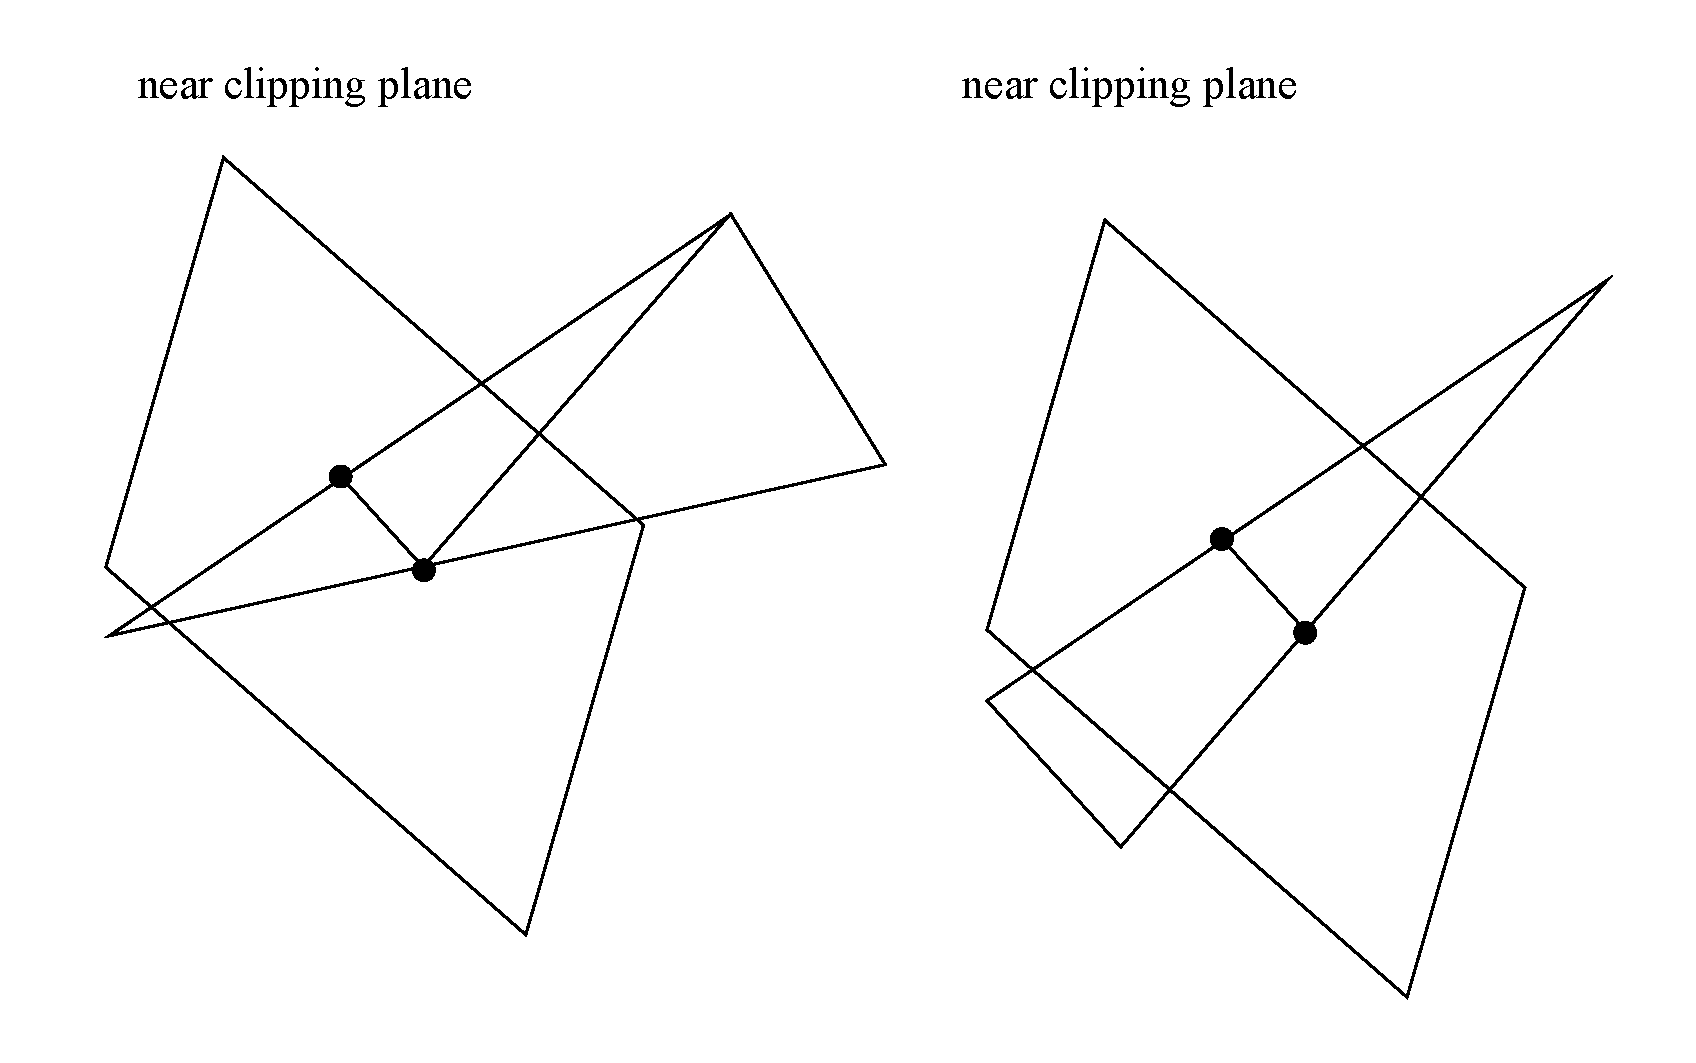
\includegraphics[width=0.7\linewidth]{imgs/triangle_clipping.pdf}
    \caption{If one or two vertices of a triangle is behind the near clipping plane, then (ideally) we would need to clip the triangle. If only one vertex is behind the clipping plane (left), then we need to clip and further split the resulting quadliteral into two triangles. If two vertices are behind the clipping plane (right), the clipped triangle is still a triangle.}
    \label{fig:triangle_clipping}
\end{figure}

\paragraph{Bonus: triangle clipping.} In practice, instead of rejecting a triangle if one or two verices are behind the near clipping plane, graphics pipelines would implement triangle clipping (\cref{fig:triangle_clipping}). As a bonus, you will implement the clipping of the triangles and render them correctly even when some vertices are behind the near clipping plane.

\section{Rendering a triangle mesh}

\section{3D transformation}

\section{Lighting}

\section{Design your own scenes}

%\bibliographystyle{plain}
%\bibliography{refs}

\end{document}
